\documentclass[a4paper,5pt]{article}
\usepackage[utf8]{inputenc}
\usepackage{indentfirst}
\usepackage[russian]{babel}
\usepackage{graphicx}
\usepackage{multicol}
\usepackage{amsmath}
\usepackage{slashbox}
\usepackage[left=2cm,right=2cm,top=2cm,bottom=2cm,bindingoffset=0cm]{geometry}
\graphicspath{{pictures/}}
\DeclareGraphicsExtensions{.pdf,.png,.jpg}
\setlength{\parindent}{1cm}
\pagestyle{empty}
\begin{document}
\begin{multicols}{2}
\fontsize{11pt}{10pt}\selectfont
\setlength{\parindent}{1cm}
\noindent если в первых двух уровни и температуры жидкостей поддерживаются постоянными.
\par \textbf{9.} Газ в цилиндрическом сосуде закрыт поршнем и разделен подвижной перегородкой на объёмы $V_1=10$ \textit{л} и $V_2=15$ \textit{л} (см. рис. 5). На какую величину сместится перегородка, если поршень изометрически сместили на $\Delta x=1$ \textit{см}?
\par \textbf{10.} Оцените, во сколько раз среднее расстояние между молекулами воды меньше среднего расстояния между молекулами водяного пара при нормальных условиях.
\par \textbf{11.}  Имеется выключатель (ключ), набор различных сопротивлений н лампочек накаливания. Составьте схему, содержащую ключ, две лампочки и, возможно, некоторые сопротивления, так, чтобы при замкнутом ключе горела одна лампочка, а при разомхнутом — только вторая.
\par \textbf{12.} Исследуйте экспериментально характер двнжения катушки по шероховатой поверхности, возникающего при сматывании нити с катушки (рис. 6). Для прозедения исследования сделайте катушку, у которой возможно изменение большого радиуса. Например, такую катушку можно изготовить из бутылки и картонных или фанерных съемных колец. \par Как зависит направление движения катушки от величины угла $\alpha$?
\par
Постройте на основании экспериментальных данных трафик зависимости угла, при котором катушка вращается на месте, от величины отношения $R/r$. Угол $\alpha$ можно измерять с помощью транспортира и отвеса. Опишите вашу экепериментальную установку. Как вы производили измерения? Какие погрешности могли исказить полученный трафик? Как можно эти погрешности уменьшить?
\par\noindent\textbf{Математика}
\par Задачи 1—5 — для седьмого класса, 4—10 — для восьмого, 7—13 — для девятого:
\par \textbf{1. } Упростить выражение:
$$
\left(\frac{2a}{2a+b}-\frac{4a^2}{4a^2+4ab+b^2}\right):
\left(\frac{2a}{4a^2-b^2}+\frac{1}{b-2a}\right).
$$
\par \textbf{2. } На школьной викторине было предложено 30 вопросов. За каждый правильный ответ участнику засчитывали 7 очков, а за \\
\noindent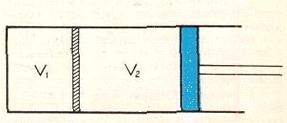
\includegraphics[scale=1]{pic1} \\
Рис. 5. \\
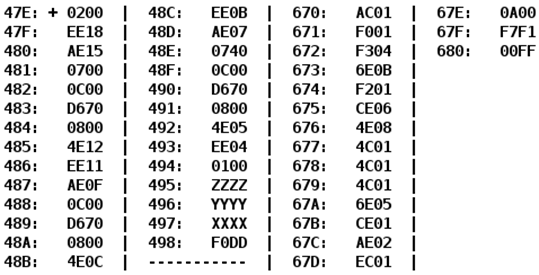
\includegraphics[scale=1]{pic2} \\
Рис. 6. \\
\\
неправильный ответ с него списывалось 12 очков. Сколько верных ответов дал ученик, если он набрал 77 очков?
\par \textbf{3. } Построить прямоугольный треугольник по катету и гипотенузе (с помощью циркуля и линейки).
\par \textbf{4. } Найти натуральные значения $n$ такие, чтобы числа $n$, $n+10$, $n+14$ все были простыми.
\par \textbf{5. } Между числами 1, 2, 3, 4, 5, 6 7, 8, 9 поставить вместо запятых пять знаков плюс и три знака минус так, чтобы получилось число 21. Сколько решений имеет задача?
\par \textbf{6. } Какое из чисел больше: $\frac{3\sqrt{7}+5\sqrt{2}}{\sqrt{5}}$ или 6?
\par \textbf{7. } В равнобедренном треугольнике центр вписанного круга делит высоту в отношении 12:5, а боковая сторона равна 60 \textit{см}. Определить основание.
\par \textbf{8. } Из пункта $A$ в пункт $B$ выехал мотоциклист, а одновременно навстречу ему из пункта $B$ в пункт $A$выехал велосепидист. Мотоциклист прибыл в пункт B через два часа после встречи с велосипидистом, а велосипедист прибыл в пункт $A$ через 4,5 часа после встречи с мотоциклистом. Сколько часов были в пути мотоциклист и велосипедист?
\par \textbf{9. } Основания трапеции равны $6\sqrt{2}$ \textit{см} и $8\sqrt{2}$ \textit{см}. Определить длину отрезка, параллельного им и делящего площадь трапеции пополам.\
\par \textbf{10. } В шахматном турнире участвовало $k$ человек — школьники и студенты. После окончания турнира оказалось, что каждый участник набрал половину своих очков в партиях против студентов. Доказать, что $k$ — полный квадрат.
\par \textbf{11. } Построить ромб, зная его диагональ и радиус вписанной окружности.
\par \textbf{12. } Решить систему уравнений:
$$
\begin{cases}
7\sqrt[3]{xy}-3\sqrt[3]{xy}=4,
\\
x+y=20.
\end{cases}
$$
\par \textbf{13.} Упростить выражение:
$$
\sqrt{a+2m\sqrt{a-m^2}}+\sqrt{a-2m\sqrt{a-m^2}}.
$$
\end{multicols}
\newpage
\begin{multicols}{2}
\noindent -----------------------------------
\par Нумерация интервалов теперь будет зависеть от знака $a$: при $a>0$ они нумеруются номерами левых концов, при $a<0$ — номерами правых концов; $y$ — число целочисленных точек в интервалах с нечетными номерами. Если мы увеличим $p$ на $4al$, то вкаждый интервал добавится точно $2l$ целых точек. Это следует из того, что при сдвиге интервала на целое число количество челых точек в нем не меняется, а на любом отрезке целочисленной длины $n$ или интервале длины $n$ с нецелочисленными концами имеется ровно $n$ целых точек (докажите!). Итак, при изменении $p$ на $p+4al$ величина $v$ изменится на четное число, а $(-1)^v$ не изменится. Значит, для всех $p$ в арифметической прогрессии $p=4aq+r$ значение $(-1)^v$ — одно и то же, и гипотеза Эйлера доказана.
\par Одноверменно указан некоторый способ выяснить, является ли $a$ квад-
\\ \noindent -------------------------------------------------------------
\par скольку в остальных случаях арифметическая прогрессия не будет содержать простых чисел. Как видно из рис. 3, число 2 является квадратичным вычетом для
\par$p=8q+1, p=8q+7,$ то есть $p=8q\pm 1.$
\par Упражнение. Покажите, что —2 есть квадратичный вычет для $p=8q+1, p=8q+3$
\par Аналогично рассматривается случай $a=\pm 3$. Приведем итоги вычислений (таблица для v):
\par
\begin{tabular}{c || c | c | c | c}
\hline
\backslashbox{a}{r} & 1 & 5 & 7 & 11 \\ \hline \hline
3 & 0 & 1 & 1 & 2 \\ \hline
—3 & 0 & 1 & 2 & 3 \\ \hline
\end{tabular}
\\
\\
\\
\\
\\
\end{multicols}
\end{document}